\documentclass[twoside]{book}

% Packages required by doxygen
\usepackage{calc}
\usepackage{doxygen}
\usepackage{graphicx}
\usepackage[utf8]{inputenc}
\usepackage{makeidx}
\usepackage{multicol}
\usepackage{multirow}
\usepackage{textcomp}
\usepackage[table]{xcolor}

% NLS support packages
\usepackage{polski}
\usepackage[T1]{fontenc}

% Font selection
\usepackage[T1]{fontenc}
\usepackage{mathptmx}
\usepackage[scaled=.90]{helvet}
\usepackage{courier}
\usepackage{amssymb}
\usepackage{sectsty}
\renewcommand{\familydefault}{\sfdefault}
\allsectionsfont{%
  \fontseries{bc}\selectfont%
  \color{darkgray}%
}
\renewcommand{\DoxyLabelFont}{%
  \fontseries{bc}\selectfont%
  \color{darkgray}%
}

% Page & text layout
\usepackage{geometry}
\geometry{%
  a4paper,%
  top=2.5cm,%
  bottom=2.5cm,%
  left=2.5cm,%
  right=2.5cm%
}
\tolerance=750
\hfuzz=15pt
\hbadness=750
\setlength{\emergencystretch}{15pt}
\setlength{\parindent}{0cm}
\setlength{\parskip}{0.2cm}
\makeatletter
\renewcommand{\paragraph}{%
  \@startsection{paragraph}{4}{0ex}{-1.0ex}{1.0ex}{%
    \normalfont\normalsize\bfseries\SS@parafont%
  }%
}
\renewcommand{\subparagraph}{%
  \@startsection{subparagraph}{5}{0ex}{-1.0ex}{1.0ex}{%
    \normalfont\normalsize\bfseries\SS@subparafont%
  }%
}
\makeatother

% Headers & footers
\usepackage{fancyhdr}
\pagestyle{fancyplain}
\fancyhead[LE]{\fancyplain{}{\bfseries\thepage}}
\fancyhead[CE]{\fancyplain{}{}}
\fancyhead[RE]{\fancyplain{}{\bfseries\leftmark}}
\fancyhead[LO]{\fancyplain{}{\bfseries\rightmark}}
\fancyhead[CO]{\fancyplain{}{}}
\fancyhead[RO]{\fancyplain{}{\bfseries\thepage}}
\fancyfoot[LE]{\fancyplain{}{}}
\fancyfoot[CE]{\fancyplain{}{}}
\fancyfoot[RE]{\fancyplain{}{\bfseries\scriptsize Wygenerowano N, 23 mar 2014 22\-:40\-:24 dla Laboratorium 4 programem Doxygen }}
\fancyfoot[LO]{\fancyplain{}{\bfseries\scriptsize Wygenerowano N, 23 mar 2014 22\-:40\-:24 dla Laboratorium 4 programem Doxygen }}
\fancyfoot[CO]{\fancyplain{}{}}
\fancyfoot[RO]{\fancyplain{}{}}
\renewcommand{\footrulewidth}{0.4pt}
\renewcommand{\chaptermark}[1]{%
  \markboth{#1}{}%
}
\renewcommand{\sectionmark}[1]{%
  \markright{\thesection\ #1}%
}

% Indices & bibliography
\usepackage{natbib}
\usepackage[titles]{tocloft}
\setcounter{tocdepth}{3}
\setcounter{secnumdepth}{5}
\makeindex

% Hyperlinks (required, but should be loaded last)
\usepackage{ifpdf}
\ifpdf
  \usepackage[pdftex,pagebackref=true]{hyperref}
\else
  \usepackage[ps2pdf,pagebackref=true]{hyperref}
\fi
\hypersetup{%
  colorlinks=true,%
  linkcolor=blue,%
  citecolor=blue,%
  unicode%
}

% Custom commands
\newcommand{\clearemptydoublepage}{%
  \newpage{\pagestyle{empty}\cleardoublepage}%
}


%===== C O N T E N T S =====

\begin{document}

% Titlepage & ToC
\hypersetup{pageanchor=false}
\pagenumbering{roman}
\begin{titlepage}
\vspace*{7cm}
\begin{center}%
{\Large Laboratorium 4 \\[1ex]\large 0.\-1 }\\
\vspace*{1cm}
{\large Wygenerowano przez Doxygen 1.8.6}\\
\vspace*{0.5cm}
{\small N, 23 mar 2014 22:40:24}\\
\end{center}
\end{titlepage}
\clearemptydoublepage
\tableofcontents
\clearemptydoublepage
\pagenumbering{arabic}
\hypersetup{pageanchor=true}

%--- Begin generated contents ---
\chapter{Dokumentacja zadania P\-A\-M\-S\-I L\-A\-B 4}
\label{index}\hypertarget{index}{}\begin{DoxyAuthor}{Author}
Justyna Klijewska 
\end{DoxyAuthor}
\begin{DoxyDate}{Date}
28.\-05.\-2014 
\end{DoxyDate}
\begin{DoxyVersion}{Version}
0.\-1 
\end{DoxyVersion}

\chapter{Indeks klas}
\section{Lista klas}
Tutaj znajdują się klasy, struktury, unie i interfejsy wraz z ich krótkimi opisami\-:\begin{DoxyCompactList}
\item\contentsline{section}{\hyperlink{class_tablica}{Tablica} }{\pageref{class_tablica}}{}
\item\contentsline{section}{\hyperlink{class_zegar}{Zegar} }{\pageref{class_zegar}}{}
\end{DoxyCompactList}

\chapter{Indeks plików}
\section{File List}
Here is a list of all files with brief descriptions\-:\begin{DoxyCompactList}
\item\contentsline{section}{C\-:/\-Users/\-Klijek/\-Documents/\-Git\-Hub/\-Pamis02/\-L\-A\-B8/prj/\hyperlink{graf_8cpp}{graf.\-cpp} }{\pageref{graf_8cpp}}{}
\item\contentsline{section}{C\-:/\-Users/\-Klijek/\-Documents/\-Git\-Hub/\-Pamis02/\-L\-A\-B8/prj/\hyperlink{graf_8hpp}{graf.\-hpp} }{\pageref{graf_8hpp}}{}
\item\contentsline{section}{C\-:/\-Users/\-Klijek/\-Documents/\-Git\-Hub/\-Pamis02/\-L\-A\-B8/prj/\hyperlink{main_8cpp}{main.\-cpp} }{\pageref{main_8cpp}}{}
\end{DoxyCompactList}

\chapter{Dokumentacja klas}
\hypertarget{class_list}{\section{Dokumentacja klasy List}
\label{class_list}\index{List@{List}}
}


{\ttfamily \#include $<$lista.\-hpp$>$}

\subsection*{Metody publiczne}
\begin{DoxyCompactItemize}
\item 
\hyperlink{class_list_a64d878a92d11f7c63c70cbe4e7dd4176}{List} ()
\item 
\hyperlink{class_list_a70aecf37bd9d779a394e4d50377fbf5f}{$\sim$\-List} ()
\item 
void \hyperlink{class_list_ae14e825ab502fe31686bf3059ed85ed0}{Isempty} ()
\item 
int \hyperlink{class_list_a00e0054a58302c9eceb94d2ca884e6c5}{Size} ()
\item 
void \hyperlink{class_list_a31fbd443a2454901d82e4baa1732fe62}{Push\-\_\-\-Front} (double number)
\item 
double \hyperlink{class_list_a60d28fbb02bd3fc770ba0627d9345dde}{Pop\-\_\-\-Front} ()
\item 
double \hyperlink{class_list_a8b06ea3ceef6bb1b261656e78e1ba6e7}{Pop\-\_\-\-Back} ()
\item 
void \hyperlink{class_list_a25ab387de5733d3a908b730877b0f260}{Show\-\_\-\-List} ()
\item 
\hyperlink{class_list}{List} \& \hyperlink{class_list_a7c478a92a9c02c8948e4495ab8e9acc1}{operator==} (\hyperlink{class_list}{List} \&lista)
\item 
\hyperlink{class_list}{List} \& \hyperlink{class_list_ae49de6522570c22c3dc2d695cbb4ecbf}{operator$\ast$} (double M)
\end{DoxyCompactItemize}


\subsection{Opis szczegółowy}


Definicja w linii 21 pliku lista.\-hpp.



\subsection{Dokumentacja konstruktora i destruktora}
\hypertarget{class_list_a64d878a92d11f7c63c70cbe4e7dd4176}{\index{List@{List}!List@{List}}
\index{List@{List}!List@{List}}
\subsubsection[{List}]{\setlength{\rightskip}{0pt plus 5cm}List\-::\-List (
\begin{DoxyParamCaption}
{}
\end{DoxyParamCaption}
)}}\label{class_list_a64d878a92d11f7c63c70cbe4e7dd4176}


Definicja w linii 9 pliku lista.\-cpp.

\hypertarget{class_list_a70aecf37bd9d779a394e4d50377fbf5f}{\index{List@{List}!$\sim$\-List@{$\sim$\-List}}
\index{$\sim$\-List@{$\sim$\-List}!List@{List}}
\subsubsection[{$\sim$\-List}]{\setlength{\rightskip}{0pt plus 5cm}List\-::$\sim$\-List (
\begin{DoxyParamCaption}
{}
\end{DoxyParamCaption}
)}}\label{class_list_a70aecf37bd9d779a394e4d50377fbf5f}


Definicja w linii 20 pliku lista.\-cpp.



\subsection{Dokumentacja funkcji składowych}
\hypertarget{class_list_ae14e825ab502fe31686bf3059ed85ed0}{\index{List@{List}!Isempty@{Isempty}}
\index{Isempty@{Isempty}!List@{List}}
\subsubsection[{Isempty}]{\setlength{\rightskip}{0pt plus 5cm}void List\-::\-Isempty (
\begin{DoxyParamCaption}
{}
\end{DoxyParamCaption}
)}}\label{class_list_ae14e825ab502fe31686bf3059ed85ed0}


Definicja w linii 36 pliku lista.\-cpp.



Oto graf wywoływań tej funkcji\-:


\hypertarget{class_list_ae49de6522570c22c3dc2d695cbb4ecbf}{\index{List@{List}!operator$\ast$@{operator$\ast$}}
\index{operator$\ast$@{operator$\ast$}!List@{List}}
\subsubsection[{operator$\ast$}]{\setlength{\rightskip}{0pt plus 5cm}{\bf List} \& List\-::operator$\ast$ (
\begin{DoxyParamCaption}
\item[{double}]{M}
\end{DoxyParamCaption}
)}}\label{class_list_ae49de6522570c22c3dc2d695cbb4ecbf}


Definicja w linii 222 pliku lista.\-cpp.

\hypertarget{class_list_a7c478a92a9c02c8948e4495ab8e9acc1}{\index{List@{List}!operator==@{operator==}}
\index{operator==@{operator==}!List@{List}}
\subsubsection[{operator==}]{\setlength{\rightskip}{0pt plus 5cm}{\bf List} \& List\-::operator== (
\begin{DoxyParamCaption}
\item[{{\bf List} \&}]{lista}
\end{DoxyParamCaption}
)}}\label{class_list_a7c478a92a9c02c8948e4495ab8e9acc1}


Definicja w linii 152 pliku lista.\-cpp.



Oto graf wywołań dla tej funkcji\-:


\hypertarget{class_list_a8b06ea3ceef6bb1b261656e78e1ba6e7}{\index{List@{List}!Pop\-\_\-\-Back@{Pop\-\_\-\-Back}}
\index{Pop\-\_\-\-Back@{Pop\-\_\-\-Back}!List@{List}}
\subsubsection[{Pop\-\_\-\-Back}]{\setlength{\rightskip}{0pt plus 5cm}double List\-::\-Pop\-\_\-\-Back (
\begin{DoxyParamCaption}
{}
\end{DoxyParamCaption}
)}}\label{class_list_a8b06ea3ceef6bb1b261656e78e1ba6e7}


Definicja w linii 101 pliku lista.\-cpp.



Oto graf wywoływań tej funkcji\-:


\hypertarget{class_list_a60d28fbb02bd3fc770ba0627d9345dde}{\index{List@{List}!Pop\-\_\-\-Front@{Pop\-\_\-\-Front}}
\index{Pop\-\_\-\-Front@{Pop\-\_\-\-Front}!List@{List}}
\subsubsection[{Pop\-\_\-\-Front}]{\setlength{\rightskip}{0pt plus 5cm}double List\-::\-Pop\-\_\-\-Front (
\begin{DoxyParamCaption}
{}
\end{DoxyParamCaption}
)}}\label{class_list_a60d28fbb02bd3fc770ba0627d9345dde}


Definicja w linii 79 pliku lista.\-cpp.



Oto graf wywoływań tej funkcji\-:


\hypertarget{class_list_a31fbd443a2454901d82e4baa1732fe62}{\index{List@{List}!Push\-\_\-\-Front@{Push\-\_\-\-Front}}
\index{Push\-\_\-\-Front@{Push\-\_\-\-Front}!List@{List}}
\subsubsection[{Push\-\_\-\-Front}]{\setlength{\rightskip}{0pt plus 5cm}void List\-::\-Push\-\_\-\-Front (
\begin{DoxyParamCaption}
\item[{double}]{number}
\end{DoxyParamCaption}
)}}\label{class_list_a31fbd443a2454901d82e4baa1732fe62}


Definicja w linii 58 pliku lista.\-cpp.



Oto graf wywoływań tej funkcji\-:


\hypertarget{class_list_a25ab387de5733d3a908b730877b0f260}{\index{List@{List}!Show\-\_\-\-List@{Show\-\_\-\-List}}
\index{Show\-\_\-\-List@{Show\-\_\-\-List}!List@{List}}
\subsubsection[{Show\-\_\-\-List}]{\setlength{\rightskip}{0pt plus 5cm}void List\-::\-Show\-\_\-\-List (
\begin{DoxyParamCaption}
{}
\end{DoxyParamCaption}
)}}\label{class_list_a25ab387de5733d3a908b730877b0f260}


Definicja w linii 126 pliku lista.\-cpp.



Oto graf wywoływań tej funkcji\-:


\hypertarget{class_list_a00e0054a58302c9eceb94d2ca884e6c5}{\index{List@{List}!Size@{Size}}
\index{Size@{Size}!List@{List}}
\subsubsection[{Size}]{\setlength{\rightskip}{0pt plus 5cm}int List\-::\-Size (
\begin{DoxyParamCaption}
{}
\end{DoxyParamCaption}
)}}\label{class_list_a00e0054a58302c9eceb94d2ca884e6c5}


Definicja w linii 47 pliku lista.\-cpp.



Oto graf wywoływań tej funkcji\-:




Dokumentacja dla tej klasy została wygenerowana z plików\-:\begin{DoxyCompactItemize}
\item 
C\-:/\-Users/\-Klijek/\-Desktop/\-L\-A\-B4/prj/\hyperlink{lista_8hpp}{lista.\-hpp}\item 
C\-:/\-Users/\-Klijek/\-Desktop/\-L\-A\-B4/prj/\hyperlink{lista_8cpp}{lista.\-cpp}\end{DoxyCompactItemize}

\hypertarget{struct_list_ele}{\section{Dokumentacja struktury List\-Ele}
\label{struct_list_ele}\index{List\-Ele@{List\-Ele}}
}


{\ttfamily \#include $<$lista.\-hpp$>$}



Diagram współpracy dla List\-Ele\-:
\subsection*{Atrybuty publiczne}
\begin{DoxyCompactItemize}
\item 
\hyperlink{struct_list_ele}{List\-Ele} $\ast$ \hyperlink{struct_list_ele_a94ce43c22a26ca3da57cdd34cd9005ad}{next}
\item 
double \hyperlink{struct_list_ele_a52bbe3635f6c0d0b095d12b97c0ee55c}{dane}
\end{DoxyCompactItemize}


\subsection{Opis szczegółowy}


Definicja w linii 10 pliku lista.\-hpp.



\subsection{Dokumentacja atrybutów składowych}
\hypertarget{struct_list_ele_a52bbe3635f6c0d0b095d12b97c0ee55c}{\index{List\-Ele@{List\-Ele}!dane@{dane}}
\index{dane@{dane}!ListEle@{List\-Ele}}
\subsubsection[{dane}]{\setlength{\rightskip}{0pt plus 5cm}double List\-Ele\-::dane}}\label{struct_list_ele_a52bbe3635f6c0d0b095d12b97c0ee55c}


Definicja w linii 13 pliku lista.\-hpp.

\hypertarget{struct_list_ele_a94ce43c22a26ca3da57cdd34cd9005ad}{\index{List\-Ele@{List\-Ele}!next@{next}}
\index{next@{next}!ListEle@{List\-Ele}}
\subsubsection[{next}]{\setlength{\rightskip}{0pt plus 5cm}{\bf List\-Ele}$\ast$ List\-Ele\-::next}}\label{struct_list_ele_a94ce43c22a26ca3da57cdd34cd9005ad}


Definicja w linii 12 pliku lista.\-hpp.



Dokumentacja dla tej struktury została wygenerowana z pliku\-:\begin{DoxyCompactItemize}
\item 
C\-:/\-Users/\-Klijek/\-Desktop/\-L\-A\-B4/prj/\hyperlink{lista_8hpp}{lista.\-hpp}\end{DoxyCompactItemize}

\hypertarget{class_queue}{\section{Dokumentacja klasy Queue}
\label{class_queue}\index{Queue@{Queue}}
}


{\ttfamily \#include $<$kolejka.\-hpp$>$}

\subsection*{Metody publiczne}
\begin{DoxyCompactItemize}
\item 
\hyperlink{class_queue_af1fd9bf4e7e72c4393f70d6cc6510e72}{Queue} (int typ)
\item 
void \hyperlink{class_queue_ad79218b6296d87515f0a487764c44111}{Enqueue} (double ele)
\item 
double \hyperlink{class_queue_af6a908c687baa28ac3237dcf22c1ba13}{Dequeue} ()
\item 
void \hyperlink{class_queue_ae671ac7c20b47b9a57eb008e1b946bfe}{Isempty} ()
\item 
int \hyperlink{class_queue_a2b28fe3446577261546f74b7bbe3ccc6}{Size} ()
\item 
void \hyperlink{class_queue_a05d02f07f4803b68cfb31c5e009b9fcc}{Q\-S} ()
\item 
void \hyperlink{class_queue_a08133cee98c6aeb1743b6dbd3e5dda91}{H\-S} ()
\item 
void \hyperlink{class_queue_aff513390c08fdd376577704be1d831c9}{M\-S} ()
\item 
void \hyperlink{class_queue_a2f80b1ea8c0af424d0153af7563e1c34}{Show} ()
\item 
\hyperlink{class_queue}{Queue} \& \hyperlink{class_queue_aef9c898949be023f99190e5f45996587}{operator==} (\hyperlink{class_queue}{Queue} \&que)
\item 
\hyperlink{class_queue}{Queue} \& \hyperlink{class_queue_a1b806694ad653ed3dd0fc48a216f97bc}{operator$\ast$} (double M)
\end{DoxyCompactItemize}


\subsection{Opis szczegółowy}


Definicja w linii 13 pliku kolejka.\-hpp.



\subsection{Dokumentacja konstruktora i destruktora}
\hypertarget{class_queue_af1fd9bf4e7e72c4393f70d6cc6510e72}{\index{Queue@{Queue}!Queue@{Queue}}
\index{Queue@{Queue}!Queue@{Queue}}
\subsubsection[{Queue}]{\setlength{\rightskip}{0pt plus 5cm}Queue\-::\-Queue (
\begin{DoxyParamCaption}
\item[{int}]{typ}
\end{DoxyParamCaption}
)\hspace{0.3cm}{\ttfamily [inline]}}}\label{class_queue_af1fd9bf4e7e72c4393f70d6cc6510e72}


Definicja w linii 22 pliku kolejka.\-hpp.



\subsection{Dokumentacja funkcji składowych}
\hypertarget{class_queue_af6a908c687baa28ac3237dcf22c1ba13}{\index{Queue@{Queue}!Dequeue@{Dequeue}}
\index{Dequeue@{Dequeue}!Queue@{Queue}}
\subsubsection[{Dequeue}]{\setlength{\rightskip}{0pt plus 5cm}double Queue\-::\-Dequeue (
\begin{DoxyParamCaption}
{}
\end{DoxyParamCaption}
)\hspace{0.3cm}{\ttfamily [inline]}}}\label{class_queue_af6a908c687baa28ac3237dcf22c1ba13}


Definicja w linii 25 pliku kolejka.\-hpp.



Oto graf wywołań dla tej funkcji\-:




Oto graf wywoływań tej funkcji\-:


\hypertarget{class_queue_ad79218b6296d87515f0a487764c44111}{\index{Queue@{Queue}!Enqueue@{Enqueue}}
\index{Enqueue@{Enqueue}!Queue@{Queue}}
\subsubsection[{Enqueue}]{\setlength{\rightskip}{0pt plus 5cm}void Queue\-::\-Enqueue (
\begin{DoxyParamCaption}
\item[{double}]{ele}
\end{DoxyParamCaption}
)\hspace{0.3cm}{\ttfamily [inline]}}}\label{class_queue_ad79218b6296d87515f0a487764c44111}


Definicja w linii 24 pliku kolejka.\-hpp.



Oto graf wywołań dla tej funkcji\-:




Oto graf wywoływań tej funkcji\-:


\hypertarget{class_queue_a08133cee98c6aeb1743b6dbd3e5dda91}{\index{Queue@{Queue}!H\-S@{H\-S}}
\index{H\-S@{H\-S}!Queue@{Queue}}
\subsubsection[{H\-S}]{\setlength{\rightskip}{0pt plus 5cm}void Queue\-::\-H\-S (
\begin{DoxyParamCaption}
{}
\end{DoxyParamCaption}
)\hspace{0.3cm}{\ttfamily [inline]}}}\label{class_queue_a08133cee98c6aeb1743b6dbd3e5dda91}


Definicja w linii 30 pliku kolejka.\-hpp.



Oto graf wywołań dla tej funkcji\-:


\hypertarget{class_queue_ae671ac7c20b47b9a57eb008e1b946bfe}{\index{Queue@{Queue}!Isempty@{Isempty}}
\index{Isempty@{Isempty}!Queue@{Queue}}
\subsubsection[{Isempty}]{\setlength{\rightskip}{0pt plus 5cm}void Queue\-::\-Isempty (
\begin{DoxyParamCaption}
{}
\end{DoxyParamCaption}
)\hspace{0.3cm}{\ttfamily [inline]}}}\label{class_queue_ae671ac7c20b47b9a57eb008e1b946bfe}


Definicja w linii 26 pliku kolejka.\-hpp.



Oto graf wywołań dla tej funkcji\-:


\hypertarget{class_queue_aff513390c08fdd376577704be1d831c9}{\index{Queue@{Queue}!M\-S@{M\-S}}
\index{M\-S@{M\-S}!Queue@{Queue}}
\subsubsection[{M\-S}]{\setlength{\rightskip}{0pt plus 5cm}void Queue\-::\-M\-S (
\begin{DoxyParamCaption}
{}
\end{DoxyParamCaption}
)\hspace{0.3cm}{\ttfamily [inline]}}}\label{class_queue_aff513390c08fdd376577704be1d831c9}


Definicja w linii 31 pliku kolejka.\-hpp.



Oto graf wywołań dla tej funkcji\-:


\hypertarget{class_queue_a1b806694ad653ed3dd0fc48a216f97bc}{\index{Queue@{Queue}!operator$\ast$@{operator$\ast$}}
\index{operator$\ast$@{operator$\ast$}!Queue@{Queue}}
\subsubsection[{operator$\ast$}]{\setlength{\rightskip}{0pt plus 5cm}{\bf Queue}\& Queue\-::operator$\ast$ (
\begin{DoxyParamCaption}
\item[{double}]{M}
\end{DoxyParamCaption}
)\hspace{0.3cm}{\ttfamily [inline]}}}\label{class_queue_a1b806694ad653ed3dd0fc48a216f97bc}


Definicja w linii 35 pliku kolejka.\-hpp.

\hypertarget{class_queue_aef9c898949be023f99190e5f45996587}{\index{Queue@{Queue}!operator==@{operator==}}
\index{operator==@{operator==}!Queue@{Queue}}
\subsubsection[{operator==}]{\setlength{\rightskip}{0pt plus 5cm}{\bf Queue}\& Queue\-::operator== (
\begin{DoxyParamCaption}
\item[{{\bf Queue} \&}]{que}
\end{DoxyParamCaption}
)\hspace{0.3cm}{\ttfamily [inline]}}}\label{class_queue_aef9c898949be023f99190e5f45996587}


Definicja w linii 34 pliku kolejka.\-hpp.

\hypertarget{class_queue_a05d02f07f4803b68cfb31c5e009b9fcc}{\index{Queue@{Queue}!Q\-S@{Q\-S}}
\index{Q\-S@{Q\-S}!Queue@{Queue}}
\subsubsection[{Q\-S}]{\setlength{\rightskip}{0pt plus 5cm}void Queue\-::\-Q\-S (
\begin{DoxyParamCaption}
{}
\end{DoxyParamCaption}
)\hspace{0.3cm}{\ttfamily [inline]}}}\label{class_queue_a05d02f07f4803b68cfb31c5e009b9fcc}


Definicja w linii 29 pliku kolejka.\-hpp.



Oto graf wywołań dla tej funkcji\-:


\hypertarget{class_queue_a2f80b1ea8c0af424d0153af7563e1c34}{\index{Queue@{Queue}!Show@{Show}}
\index{Show@{Show}!Queue@{Queue}}
\subsubsection[{Show}]{\setlength{\rightskip}{0pt plus 5cm}void Queue\-::\-Show (
\begin{DoxyParamCaption}
{}
\end{DoxyParamCaption}
)\hspace{0.3cm}{\ttfamily [inline]}}}\label{class_queue_a2f80b1ea8c0af424d0153af7563e1c34}


Definicja w linii 33 pliku kolejka.\-hpp.



Oto graf wywołań dla tej funkcji\-:


\hypertarget{class_queue_a2b28fe3446577261546f74b7bbe3ccc6}{\index{Queue@{Queue}!Size@{Size}}
\index{Size@{Size}!Queue@{Queue}}
\subsubsection[{Size}]{\setlength{\rightskip}{0pt plus 5cm}int Queue\-::\-Size (
\begin{DoxyParamCaption}
{}
\end{DoxyParamCaption}
)\hspace{0.3cm}{\ttfamily [inline]}}}\label{class_queue_a2b28fe3446577261546f74b7bbe3ccc6}


Definicja w linii 27 pliku kolejka.\-hpp.



Oto graf wywołań dla tej funkcji\-:




Oto graf wywoływań tej funkcji\-:




Dokumentacja dla tej klasy została wygenerowana z pliku\-:\begin{DoxyCompactItemize}
\item 
C\-:/\-Users/\-Klijek/\-Desktop/\-L\-A\-B4/prj/\hyperlink{kolejka_8hpp}{kolejka.\-hpp}\end{DoxyCompactItemize}

\hypertarget{class_stos}{\section{Dokumentacja klasy Stos}
\label{class_stos}\index{Stos@{Stos}}
}


{\ttfamily \#include $<$stos.\-hpp$>$}

\subsection*{Metody publiczne}
\begin{DoxyCompactItemize}
\item 
\hyperlink{class_stos_a9f1a0e5eb781e7296493d9c61f6ce2e2}{Stos} (int typ)
\item 
void \hyperlink{class_stos_af8c0c485dceb28e986cdc93e933ec365}{Push} (double ele)
\item 
double \hyperlink{class_stos_a620d6e49f74becaed97de2a911ef051c}{Pop} ()
\item 
void \hyperlink{class_stos_a8e559abb36abb64c458bdc281e273cba}{Isempty} ()
\item 
int \hyperlink{class_stos_a9861291fa460528db0dea0262bf88f69}{Size} ()
\item 
void \hyperlink{class_stos_a94b800e273d51af77ae4fcf88b3134e4}{Q\-S} ()
\item 
void \hyperlink{class_stos_a0e531afe4371783988c3ba470c04f5df}{H\-S} ()
\item 
void \hyperlink{class_stos_a16e80bfd5b01cc6febec3a94269daea5}{M\-S} ()
\item 
void \hyperlink{class_stos_abfb03d80298013a2792bde2fd89c3863}{Show} ()
\item 
\hyperlink{class_stos}{Stos} \& \hyperlink{class_stos_a46c03bf71cc3b8abc5537a5a408c43e8}{operator==} (\hyperlink{class_stos}{Stos} \&sto)
\item 
\hyperlink{class_stos}{Stos} \& \hyperlink{class_stos_a1a82883d837c3c63c3621e284c707304}{operator$\ast$} (double M)
\end{DoxyCompactItemize}


\subsection{Opis szczegółowy}


Definicja w linii 17 pliku stos.\-hpp.



\subsection{Dokumentacja konstruktora i destruktora}
\hypertarget{class_stos_a9f1a0e5eb781e7296493d9c61f6ce2e2}{\index{Stos@{Stos}!Stos@{Stos}}
\index{Stos@{Stos}!Stos@{Stos}}
\subsubsection[{Stos}]{\setlength{\rightskip}{0pt plus 5cm}Stos\-::\-Stos (
\begin{DoxyParamCaption}
\item[{int}]{typ}
\end{DoxyParamCaption}
)\hspace{0.3cm}{\ttfamily [inline]}}}\label{class_stos_a9f1a0e5eb781e7296493d9c61f6ce2e2}


Definicja w linii 26 pliku stos.\-hpp.



\subsection{Dokumentacja funkcji składowych}
\hypertarget{class_stos_a0e531afe4371783988c3ba470c04f5df}{\index{Stos@{Stos}!H\-S@{H\-S}}
\index{H\-S@{H\-S}!Stos@{Stos}}
\subsubsection[{H\-S}]{\setlength{\rightskip}{0pt plus 5cm}void Stos\-::\-H\-S (
\begin{DoxyParamCaption}
{}
\end{DoxyParamCaption}
)\hspace{0.3cm}{\ttfamily [inline]}}}\label{class_stos_a0e531afe4371783988c3ba470c04f5df}


Definicja w linii 34 pliku stos.\-hpp.



Oto graf wywołań dla tej funkcji\-:




Oto graf wywoływań tej funkcji\-:


\hypertarget{class_stos_a8e559abb36abb64c458bdc281e273cba}{\index{Stos@{Stos}!Isempty@{Isempty}}
\index{Isempty@{Isempty}!Stos@{Stos}}
\subsubsection[{Isempty}]{\setlength{\rightskip}{0pt plus 5cm}void Stos\-::\-Isempty (
\begin{DoxyParamCaption}
{}
\end{DoxyParamCaption}
)\hspace{0.3cm}{\ttfamily [inline]}}}\label{class_stos_a8e559abb36abb64c458bdc281e273cba}


Definicja w linii 30 pliku stos.\-hpp.



Oto graf wywołań dla tej funkcji\-:


\hypertarget{class_stos_a16e80bfd5b01cc6febec3a94269daea5}{\index{Stos@{Stos}!M\-S@{M\-S}}
\index{M\-S@{M\-S}!Stos@{Stos}}
\subsubsection[{M\-S}]{\setlength{\rightskip}{0pt plus 5cm}void Stos\-::\-M\-S (
\begin{DoxyParamCaption}
{}
\end{DoxyParamCaption}
)\hspace{0.3cm}{\ttfamily [inline]}}}\label{class_stos_a16e80bfd5b01cc6febec3a94269daea5}


Definicja w linii 35 pliku stos.\-hpp.



Oto graf wywołań dla tej funkcji\-:


\hypertarget{class_stos_a1a82883d837c3c63c3621e284c707304}{\index{Stos@{Stos}!operator$\ast$@{operator$\ast$}}
\index{operator$\ast$@{operator$\ast$}!Stos@{Stos}}
\subsubsection[{operator$\ast$}]{\setlength{\rightskip}{0pt plus 5cm}{\bf Stos}\& Stos\-::operator$\ast$ (
\begin{DoxyParamCaption}
\item[{double}]{M}
\end{DoxyParamCaption}
)\hspace{0.3cm}{\ttfamily [inline]}}}\label{class_stos_a1a82883d837c3c63c3621e284c707304}


Definicja w linii 39 pliku stos.\-hpp.

\hypertarget{class_stos_a46c03bf71cc3b8abc5537a5a408c43e8}{\index{Stos@{Stos}!operator==@{operator==}}
\index{operator==@{operator==}!Stos@{Stos}}
\subsubsection[{operator==}]{\setlength{\rightskip}{0pt plus 5cm}{\bf Stos}\& Stos\-::operator== (
\begin{DoxyParamCaption}
\item[{{\bf Stos} \&}]{sto}
\end{DoxyParamCaption}
)\hspace{0.3cm}{\ttfamily [inline]}}}\label{class_stos_a46c03bf71cc3b8abc5537a5a408c43e8}


Definicja w linii 38 pliku stos.\-hpp.

\hypertarget{class_stos_a620d6e49f74becaed97de2a911ef051c}{\index{Stos@{Stos}!Pop@{Pop}}
\index{Pop@{Pop}!Stos@{Stos}}
\subsubsection[{Pop}]{\setlength{\rightskip}{0pt plus 5cm}double Stos\-::\-Pop (
\begin{DoxyParamCaption}
{}
\end{DoxyParamCaption}
)\hspace{0.3cm}{\ttfamily [inline]}}}\label{class_stos_a620d6e49f74becaed97de2a911ef051c}


Definicja w linii 29 pliku stos.\-hpp.



Oto graf wywołań dla tej funkcji\-:




Oto graf wywoływań tej funkcji\-:


\hypertarget{class_stos_af8c0c485dceb28e986cdc93e933ec365}{\index{Stos@{Stos}!Push@{Push}}
\index{Push@{Push}!Stos@{Stos}}
\subsubsection[{Push}]{\setlength{\rightskip}{0pt plus 5cm}void Stos\-::\-Push (
\begin{DoxyParamCaption}
\item[{double}]{ele}
\end{DoxyParamCaption}
)\hspace{0.3cm}{\ttfamily [inline]}}}\label{class_stos_af8c0c485dceb28e986cdc93e933ec365}


Definicja w linii 28 pliku stos.\-hpp.



Oto graf wywołań dla tej funkcji\-:




Oto graf wywoływań tej funkcji\-:


\hypertarget{class_stos_a94b800e273d51af77ae4fcf88b3134e4}{\index{Stos@{Stos}!Q\-S@{Q\-S}}
\index{Q\-S@{Q\-S}!Stos@{Stos}}
\subsubsection[{Q\-S}]{\setlength{\rightskip}{0pt plus 5cm}void Stos\-::\-Q\-S (
\begin{DoxyParamCaption}
{}
\end{DoxyParamCaption}
)\hspace{0.3cm}{\ttfamily [inline]}}}\label{class_stos_a94b800e273d51af77ae4fcf88b3134e4}


Definicja w linii 33 pliku stos.\-hpp.



Oto graf wywołań dla tej funkcji\-:


\hypertarget{class_stos_abfb03d80298013a2792bde2fd89c3863}{\index{Stos@{Stos}!Show@{Show}}
\index{Show@{Show}!Stos@{Stos}}
\subsubsection[{Show}]{\setlength{\rightskip}{0pt plus 5cm}void Stos\-::\-Show (
\begin{DoxyParamCaption}
{}
\end{DoxyParamCaption}
)\hspace{0.3cm}{\ttfamily [inline]}}}\label{class_stos_abfb03d80298013a2792bde2fd89c3863}


Definicja w linii 37 pliku stos.\-hpp.



Oto graf wywołań dla tej funkcji\-:


\hypertarget{class_stos_a9861291fa460528db0dea0262bf88f69}{\index{Stos@{Stos}!Size@{Size}}
\index{Size@{Size}!Stos@{Stos}}
\subsubsection[{Size}]{\setlength{\rightskip}{0pt plus 5cm}int Stos\-::\-Size (
\begin{DoxyParamCaption}
{}
\end{DoxyParamCaption}
)\hspace{0.3cm}{\ttfamily [inline]}}}\label{class_stos_a9861291fa460528db0dea0262bf88f69}


Definicja w linii 31 pliku stos.\-hpp.



Oto graf wywołań dla tej funkcji\-:




Oto graf wywoływań tej funkcji\-:




Dokumentacja dla tej klasy została wygenerowana z pliku\-:\begin{DoxyCompactItemize}
\item 
C\-:/\-Users/\-Klijek/\-Desktop/\-L\-A\-B4/prj/\hyperlink{stos_8hpp}{stos.\-hpp}\end{DoxyCompactItemize}

\hypertarget{class_tablica}{\section{Dokumentacja klasy Tablica}
\label{class_tablica}\index{Tablica@{Tablica}}
}


{\ttfamily \#include $<$tablica.\-hpp$>$}

\subsection*{Metody publiczne}
\begin{DoxyCompactItemize}
\item 
\hyperlink{class_tablica_a5f484e7b0478e1ff9b62e894f9d7b28d}{Tablica} ()
\item 
void \hyperlink{class_tablica_ae1af903a66629cd0d522eb9f2fd13116}{Push} (double ele)
\item 
double \hyperlink{class_tablica_a6153881ffda3f5361c2d664622a4eff4}{Pop} ()
\item 
double \hyperlink{class_tablica_a899c8e69cb97bd027c1c05140cd304ec}{Pop\-\_\-\-Back} ()
\item 
int \hyperlink{class_tablica_a8598f952095406441bfd2d20e76f175c}{Size} ()
\item 
void \hyperlink{class_tablica_a08b59415756d2dc7da781124809d8eb4}{Isempty} ()
\item 
void \hyperlink{class_tablica_a06c551a7e0220dde2f29cce06fb96209}{Show\-\_\-\-Tab} ()
\item 
\hyperlink{class_tablica}{Tablica} \hyperlink{class_tablica_a15c072e7160bfbdbc5d103cf0ebd6e76}{operator+} (\hyperlink{class_tablica}{Tablica} \&T2)
\item 
\hyperlink{class_tablica}{Tablica} \hyperlink{class_tablica_acabfd453d919950051b8a9cf4aac642e}{operator$\ast$} (double M)
\item 
\hyperlink{class_tablica}{Tablica} \hyperlink{class_tablica_a53bd7c9853f01a78ba2aff61ece4ccbf}{operator=} (\hyperlink{class_tablica}{Tablica} \&T2)
\item 
\hyperlink{class_tablica}{Tablica} \hyperlink{class_tablica_ae5d9fdf31df882eae683abc89fec01ad}{operator==} (\hyperlink{class_tablica}{Tablica} \&T2)
\end{DoxyCompactItemize}
\subsection*{Przyjaciele}
\begin{DoxyCompactItemize}
\item 
void \hyperlink{class_tablica_a17e08e601d94bc6fce93c91bd574e717}{Quick\-\_\-\-Sort} (\hyperlink{class_tablica}{Tablica} \&T, int left, int right)
\item 
void \hyperlink{class_tablica_a7ac406a30a3a7a46d498f05bb173809c}{Heap\-\_\-\-Sort} (\hyperlink{class_tablica}{Tablica} \&T)
\item 
void \hyperlink{class_tablica_ae6edf270c00af312bbafffc1955450cc}{Merge} (\hyperlink{class_tablica}{Tablica} \&T, int left, int cent, int right)
\end{DoxyCompactItemize}


\subsection{Opis szczegółowy}


Definicja w linii 14 pliku tablica.\-hpp.



\subsection{Dokumentacja konstruktora i destruktora}
\hypertarget{class_tablica_a5f484e7b0478e1ff9b62e894f9d7b28d}{\index{Tablica@{Tablica}!Tablica@{Tablica}}
\index{Tablica@{Tablica}!Tablica@{Tablica}}
\subsubsection[{Tablica}]{\setlength{\rightskip}{0pt plus 5cm}Tablica\-::\-Tablica (
\begin{DoxyParamCaption}
{}
\end{DoxyParamCaption}
)\hspace{0.3cm}{\ttfamily [inline]}}}\label{class_tablica_a5f484e7b0478e1ff9b62e894f9d7b28d}


Definicja w linii 20 pliku tablica.\-hpp.



\subsection{Dokumentacja funkcji składowych}
\hypertarget{class_tablica_a08b59415756d2dc7da781124809d8eb4}{\index{Tablica@{Tablica}!Isempty@{Isempty}}
\index{Isempty@{Isempty}!Tablica@{Tablica}}
\subsubsection[{Isempty}]{\setlength{\rightskip}{0pt plus 5cm}void Tablica\-::\-Isempty (
\begin{DoxyParamCaption}
{}
\end{DoxyParamCaption}
)}}\label{class_tablica_a08b59415756d2dc7da781124809d8eb4}


Definicja w linii 98 pliku tablica.\-cpp.



Oto graf wywoływań tej funkcji\-:


\hypertarget{class_tablica_acabfd453d919950051b8a9cf4aac642e}{\index{Tablica@{Tablica}!operator$\ast$@{operator$\ast$}}
\index{operator$\ast$@{operator$\ast$}!Tablica@{Tablica}}
\subsubsection[{operator$\ast$}]{\setlength{\rightskip}{0pt plus 5cm}{\bf Tablica} Tablica\-::operator$\ast$ (
\begin{DoxyParamCaption}
\item[{double}]{M}
\end{DoxyParamCaption}
)}}\label{class_tablica_acabfd453d919950051b8a9cf4aac642e}


Definicja w linii 264 pliku tablica.\-cpp.

\hypertarget{class_tablica_a15c072e7160bfbdbc5d103cf0ebd6e76}{\index{Tablica@{Tablica}!operator+@{operator+}}
\index{operator+@{operator+}!Tablica@{Tablica}}
\subsubsection[{operator+}]{\setlength{\rightskip}{0pt plus 5cm}{\bf Tablica} Tablica\-::operator+ (
\begin{DoxyParamCaption}
\item[{{\bf Tablica} \&}]{T2}
\end{DoxyParamCaption}
)}}\label{class_tablica_a15c072e7160bfbdbc5d103cf0ebd6e76}


Definicja w linii 194 pliku tablica.\-cpp.

\hypertarget{class_tablica_a53bd7c9853f01a78ba2aff61ece4ccbf}{\index{Tablica@{Tablica}!operator=@{operator=}}
\index{operator=@{operator=}!Tablica@{Tablica}}
\subsubsection[{operator=}]{\setlength{\rightskip}{0pt plus 5cm}{\bf Tablica} Tablica\-::operator= (
\begin{DoxyParamCaption}
\item[{{\bf Tablica} \&}]{T2}
\end{DoxyParamCaption}
)}}\label{class_tablica_a53bd7c9853f01a78ba2aff61ece4ccbf}


Definicja w linii 209 pliku tablica.\-cpp.

\hypertarget{class_tablica_ae5d9fdf31df882eae683abc89fec01ad}{\index{Tablica@{Tablica}!operator==@{operator==}}
\index{operator==@{operator==}!Tablica@{Tablica}}
\subsubsection[{operator==}]{\setlength{\rightskip}{0pt plus 5cm}{\bf Tablica} Tablica\-::operator== (
\begin{DoxyParamCaption}
\item[{{\bf Tablica} \&}]{T2}
\end{DoxyParamCaption}
)}}\label{class_tablica_ae5d9fdf31df882eae683abc89fec01ad}


Definicja w linii 220 pliku tablica.\-cpp.

\hypertarget{class_tablica_a6153881ffda3f5361c2d664622a4eff4}{\index{Tablica@{Tablica}!Pop@{Pop}}
\index{Pop@{Pop}!Tablica@{Tablica}}
\subsubsection[{Pop}]{\setlength{\rightskip}{0pt plus 5cm}double Tablica\-::\-Pop (
\begin{DoxyParamCaption}
{}
\end{DoxyParamCaption}
)}}\label{class_tablica_a6153881ffda3f5361c2d664622a4eff4}


Definicja w linii 33 pliku tablica.\-cpp.



Oto graf wywoływań tej funkcji\-:


\hypertarget{class_tablica_a899c8e69cb97bd027c1c05140cd304ec}{\index{Tablica@{Tablica}!Pop\-\_\-\-Back@{Pop\-\_\-\-Back}}
\index{Pop\-\_\-\-Back@{Pop\-\_\-\-Back}!Tablica@{Tablica}}
\subsubsection[{Pop\-\_\-\-Back}]{\setlength{\rightskip}{0pt plus 5cm}double Tablica\-::\-Pop\-\_\-\-Back (
\begin{DoxyParamCaption}
{}
\end{DoxyParamCaption}
)}}\label{class_tablica_a899c8e69cb97bd027c1c05140cd304ec}


Definicja w linii 59 pliku tablica.\-cpp.



Oto graf wywoływań tej funkcji\-:


\hypertarget{class_tablica_ae1af903a66629cd0d522eb9f2fd13116}{\index{Tablica@{Tablica}!Push@{Push}}
\index{Push@{Push}!Tablica@{Tablica}}
\subsubsection[{Push}]{\setlength{\rightskip}{0pt plus 5cm}void Tablica\-::\-Push (
\begin{DoxyParamCaption}
\item[{double}]{ele}
\end{DoxyParamCaption}
)}}\label{class_tablica_ae1af903a66629cd0d522eb9f2fd13116}


Definicja w linii 17 pliku tablica.\-cpp.



Oto graf wywoływań tej funkcji\-:


\hypertarget{class_tablica_a06c551a7e0220dde2f29cce06fb96209}{\index{Tablica@{Tablica}!Show\-\_\-\-Tab@{Show\-\_\-\-Tab}}
\index{Show\-\_\-\-Tab@{Show\-\_\-\-Tab}!Tablica@{Tablica}}
\subsubsection[{Show\-\_\-\-Tab}]{\setlength{\rightskip}{0pt plus 5cm}void Tablica\-::\-Show\-\_\-\-Tab (
\begin{DoxyParamCaption}
{}
\end{DoxyParamCaption}
)}}\label{class_tablica_a06c551a7e0220dde2f29cce06fb96209}


Definicja w linii 167 pliku tablica.\-cpp.



Oto graf wywoływań tej funkcji\-:


\hypertarget{class_tablica_a8598f952095406441bfd2d20e76f175c}{\index{Tablica@{Tablica}!Size@{Size}}
\index{Size@{Size}!Tablica@{Tablica}}
\subsubsection[{Size}]{\setlength{\rightskip}{0pt plus 5cm}int Tablica\-::\-Size (
\begin{DoxyParamCaption}
{}
\end{DoxyParamCaption}
)}}\label{class_tablica_a8598f952095406441bfd2d20e76f175c}


Definicja w linii 86 pliku tablica.\-cpp.



Oto graf wywoływań tej funkcji\-:




\subsection{Dokumentacja przyjaciół i funkcji związanych}
\hypertarget{class_tablica_a7ac406a30a3a7a46d498f05bb173809c}{\index{Tablica@{Tablica}!Heap\-\_\-\-Sort@{Heap\-\_\-\-Sort}}
\index{Heap\-\_\-\-Sort@{Heap\-\_\-\-Sort}!Tablica@{Tablica}}
\subsubsection[{Heap\-\_\-\-Sort}]{\setlength{\rightskip}{0pt plus 5cm}void Heap\-\_\-\-Sort (
\begin{DoxyParamCaption}
\item[{{\bf Tablica} \&}]{T}
\end{DoxyParamCaption}
)\hspace{0.3cm}{\ttfamily [friend]}}}\label{class_tablica_a7ac406a30a3a7a46d498f05bb173809c}


Definicja w linii 34 pliku sort.\-cpp.

\hypertarget{class_tablica_ae6edf270c00af312bbafffc1955450cc}{\index{Tablica@{Tablica}!Merge@{Merge}}
\index{Merge@{Merge}!Tablica@{Tablica}}
\subsubsection[{Merge}]{\setlength{\rightskip}{0pt plus 5cm}void Merge (
\begin{DoxyParamCaption}
\item[{{\bf Tablica} \&}]{T, }
\item[{int}]{left, }
\item[{int}]{cent, }
\item[{int}]{right}
\end{DoxyParamCaption}
)\hspace{0.3cm}{\ttfamily [friend]}}}\label{class_tablica_ae6edf270c00af312bbafffc1955450cc}


Definicja w linii 79 pliku sort.\-cpp.

\hypertarget{class_tablica_a17e08e601d94bc6fce93c91bd574e717}{\index{Tablica@{Tablica}!Quick\-\_\-\-Sort@{Quick\-\_\-\-Sort}}
\index{Quick\-\_\-\-Sort@{Quick\-\_\-\-Sort}!Tablica@{Tablica}}
\subsubsection[{Quick\-\_\-\-Sort}]{\setlength{\rightskip}{0pt plus 5cm}void Quick\-\_\-\-Sort (
\begin{DoxyParamCaption}
\item[{{\bf Tablica} \&}]{T, }
\item[{int}]{left, }
\item[{int}]{right}
\end{DoxyParamCaption}
)\hspace{0.3cm}{\ttfamily [friend]}}}\label{class_tablica_a17e08e601d94bc6fce93c91bd574e717}


Definicja w linii 3 pliku sort.\-cpp.



Dokumentacja dla tej klasy została wygenerowana z plików\-:\begin{DoxyCompactItemize}
\item 
C\-:/\-Users/\-Klijek/\-Desktop/\-L\-A\-B4/prj/\hyperlink{tablica_8hpp}{tablica.\-hpp}\item 
C\-:/\-Users/\-Klijek/\-Desktop/\-L\-A\-B4/prj/\hyperlink{tablica_8cpp}{tablica.\-cpp}\end{DoxyCompactItemize}

\hypertarget{class_zegar}{\section{Dokumentacja klasy Zegar}
\label{class_zegar}\index{Zegar@{Zegar}}
}


{\ttfamily \#include $<$zegar.\-hpp$>$}

\subsection*{Metody publiczne}
\begin{DoxyCompactItemize}
\item 
void \hyperlink{class_zegar_af747dc3a9d58207618ec877990900b80}{Start} ()
\item 
void \hyperlink{class_zegar_a8a88ddd1aa0768bfbe37217e32a01da0}{Koniec} ()
\item 
void \hyperlink{class_zegar_a659d8f393442747d17aba3a5f6533c29}{Wynik} ()
\end{DoxyCompactItemize}


\subsection{Opis szczegółowy}


Definicja w linii 16 pliku zegar.\-hpp.



\subsection{Dokumentacja funkcji składowych}
\hypertarget{class_zegar_a8a88ddd1aa0768bfbe37217e32a01da0}{\index{Zegar@{Zegar}!Koniec@{Koniec}}
\index{Koniec@{Koniec}!Zegar@{Zegar}}
\subsubsection[{Koniec}]{\setlength{\rightskip}{0pt plus 5cm}void Zegar\-::\-Koniec (
\begin{DoxyParamCaption}
{}
\end{DoxyParamCaption}
)}}\label{class_zegar_a8a88ddd1aa0768bfbe37217e32a01da0}


Definicja w linii 20 pliku zegar.\-cpp.



Oto graf wywoływań tej funkcji\-:


\hypertarget{class_zegar_af747dc3a9d58207618ec877990900b80}{\index{Zegar@{Zegar}!Start@{Start}}
\index{Start@{Start}!Zegar@{Zegar}}
\subsubsection[{Start}]{\setlength{\rightskip}{0pt plus 5cm}void Zegar\-::\-Start (
\begin{DoxyParamCaption}
{}
\end{DoxyParamCaption}
)}}\label{class_zegar_af747dc3a9d58207618ec877990900b80}


Definicja w linii 9 pliku zegar.\-cpp.



Oto graf wywoływań tej funkcji\-:


\hypertarget{class_zegar_a659d8f393442747d17aba3a5f6533c29}{\index{Zegar@{Zegar}!Wynik@{Wynik}}
\index{Wynik@{Wynik}!Zegar@{Zegar}}
\subsubsection[{Wynik}]{\setlength{\rightskip}{0pt plus 5cm}void Zegar\-::\-Wynik (
\begin{DoxyParamCaption}
{}
\end{DoxyParamCaption}
)}}\label{class_zegar_a659d8f393442747d17aba3a5f6533c29}


Definicja w linii 36 pliku zegar.\-cpp.



Oto graf wywoływań tej funkcji\-:




Dokumentacja dla tej klasy została wygenerowana z plików\-:\begin{DoxyCompactItemize}
\item 
C\-:/\-Users/\-Klijek/\-Desktop/\-L\-A\-B4/prj/\hyperlink{zegar_8hpp}{zegar.\-hpp}\item 
C\-:/\-Users/\-Klijek/\-Desktop/\-L\-A\-B4/prj/\hyperlink{zegar_8cpp}{zegar.\-cpp}\end{DoxyCompactItemize}

\chapter{Dokumentacja plików}
\hypertarget{kolejka_8hpp}{\section{Dokumentacja pliku C\-:/\-Users/\-Klijek/\-Desktop/\-L\-A\-B4/prj/kolejka.hpp}
\label{kolejka_8hpp}\index{C\-:/\-Users/\-Klijek/\-Desktop/\-L\-A\-B4/prj/kolejka.\-hpp@{C\-:/\-Users/\-Klijek/\-Desktop/\-L\-A\-B4/prj/kolejka.\-hpp}}
}


Definicja klasy \hyperlink{class_queue}{Queue}.  


{\ttfamily \#include \char`\"{}tablica.\-hpp\char`\"{}}\\*
{\ttfamily \#include \char`\"{}lista.\-hpp\char`\"{}}\\*
Wykres zależności załączania dla kolejka.\-hpp\-:
Ten wykres pokazuje, które pliki bezpośrednio lub pośrednio załączają ten plik\-:
\subsection*{Komponenty}
\begin{DoxyCompactItemize}
\item 
class \hyperlink{class_queue}{Queue}
\end{DoxyCompactItemize}


\subsection{Opis szczegółowy}
Definicja klasy \hyperlink{class_queue}{Queue}. Klasa odpowiadaj�ca za metody wykonywane na tablicy takie jak\-: Enqueue, Dequeue, Isempty, Size, Show, operatory\-: == $\ast$ 

Definicja w pliku \hyperlink{kolejka_8hpp_source}{kolejka.\-hpp}.


\hypertarget{lista_8cpp}{\section{Dokumentacja pliku C\-:/\-Users/\-Klijek/\-Desktop/\-L\-A\-B4/prj/lista.cpp}
\label{lista_8cpp}\index{C\-:/\-Users/\-Klijek/\-Desktop/\-L\-A\-B4/prj/lista.\-cpp@{C\-:/\-Users/\-Klijek/\-Desktop/\-L\-A\-B4/prj/lista.\-cpp}}
}


Definicja konstruktora \hyperlink{class_list}{List}.  


{\ttfamily \#include \char`\"{}lista.\-hpp\char`\"{}}\\*
Wykres zależności załączania dla lista.\-cpp\-:


\subsection{Opis szczegółowy}
Definicja konstruktora \hyperlink{class_list}{List}. Przeciazenie operatora$\ast$.

Przeciazenie operatora ==.

Definicja konstruktora Show\-\_\-\-List.

Definicja konstruktora Pop\-\_\-\-Back.

Definicja konstruktora Pop\-\_\-\-Front.

Definicja konstruktora Push\-\_\-\-Front.

Definicja konstruktora Size.

Definicja konstruktora Isempty.

Definicja destruktora \hyperlink{class_list}{List}.

Prztwarza obiekt do znaczniku front i back, przypisuje N\-U\-L\-L i liczy ile el. ma lisya

Usuwa wszystkie elementy

Sprawdza czy lista jest pusta

Rozmiar listy

Dodawanie na poczatek

Jest to dla stosu. Dodaje na poczatek.

Jest to dla kolejki. Dodaje na koniec.

Pokazuje liste.

sprawdzanie czy nie sa puste, jezeli nie to\-: 1-\/ 1$>$2 wykonywany 1 if 2$>$1 drugi if else kiedy takie same

Przeciazenie operatora$\ast$ 

Definicja w pliku \hyperlink{lista_8cpp_source}{lista.\-cpp}.


\hypertarget{lista_8hpp}{\section{Dokumentacja pliku C\-:/\-Users/\-Klijek/\-Desktop/\-L\-A\-B4/prj/lista.hpp}
\label{lista_8hpp}\index{C\-:/\-Users/\-Klijek/\-Desktop/\-L\-A\-B4/prj/lista.\-hpp@{C\-:/\-Users/\-Klijek/\-Desktop/\-L\-A\-B4/prj/lista.\-hpp}}
}


Definicja Struktury \hyperlink{struct_list_ele}{List\-Ele}.  


{\ttfamily \#include $<$iostream$>$}\\*
Wykres zależności załączania dla lista.\-hpp\-:
Ten wykres pokazuje, które pliki bezpośrednio lub pośrednio załączają ten plik\-:
\subsection*{Komponenty}
\begin{DoxyCompactItemize}
\item 
struct \hyperlink{struct_list_ele}{List\-Ele}
\item 
class \hyperlink{class_list}{List}
\end{DoxyCompactItemize}


\subsection{Opis szczegółowy}
Definicja Struktury \hyperlink{struct_list_ele}{List\-Ele}. Definicja klasy Lista.

Struktura, w kt�rej zdefiniowany jest wskaznik na kolejny element listy oraz zmienna dane, ktora przechowuje dane w tym elemencie

Klasa zawira wska�niki na 1 i ostani element listy )(front, back) oraz metody takie jak\-: is empty, size, push, pop show. 

Definicja w pliku \hyperlink{lista_8hpp_source}{lista.\-hpp}.


\hypertarget{main_8cpp}{\section{Dokumentacja pliku C\-:/\-Users/\-Klijek/\-Desktop/\-L\-A\-B6/prj/main.cpp}
\label{main_8cpp}\index{C\-:/\-Users/\-Klijek/\-Desktop/\-L\-A\-B6/prj/main.\-cpp@{C\-:/\-Users/\-Klijek/\-Desktop/\-L\-A\-B6/prj/main.\-cpp}}
}
{\ttfamily \#include $<$iostream$>$}\\*
{\ttfamily \#include $<$string$>$}\\*
{\ttfamily \#include \char`\"{}tab\-Aso.\-hpp\char`\"{}}\\*
Wykres zależności załączania dla main.\-cpp\-:
\subsection*{Funkcje}
\begin{DoxyCompactItemize}
\item 
int \hyperlink{main_8cpp_ae66f6b31b5ad750f1fe042a706a4e3d4}{main} ()
\end{DoxyCompactItemize}


\subsection{Dokumentacja funkcji}
\hypertarget{main_8cpp_ae66f6b31b5ad750f1fe042a706a4e3d4}{\index{main.\-cpp@{main.\-cpp}!main@{main}}
\index{main@{main}!main.cpp@{main.\-cpp}}
\subsubsection[{main}]{\setlength{\rightskip}{0pt plus 5cm}int main (
\begin{DoxyParamCaption}
{}
\end{DoxyParamCaption}
)}}\label{main_8cpp_ae66f6b31b5ad750f1fe042a706a4e3d4}
Main

Przykladowe operacje na tablicy alokacyjnej. Wyswietlanie operacji.

Definicja w linii 13 pliku main.\-cpp.



Oto graf wywołań dla tej funkcji\-:



\hypertarget{plik_8cpp}{\section{C\-:/\-Users/\-Klijek/\-Desktop/\-Czyste zło/\-N\-W\-P (1)/prj/plik.cpp File Reference}
\label{plik_8cpp}\index{C\-:/\-Users/\-Klijek/\-Desktop/\-Czyste zło/\-N\-W\-P (1)/prj/plik.\-cpp@{C\-:/\-Users/\-Klijek/\-Desktop/\-Czyste zło/\-N\-W\-P (1)/prj/plik.\-cpp}}
}
{\ttfamily \#include \char`\"{}plik.\-hpp\char`\"{}}\\*
Include dependency graph for plik.\-cpp\-:
\subsection*{Functions}
\begin{DoxyCompactItemize}
\item 
bool \hyperlink{plik_8cpp_a25526dd8d4962bb270d7624259908375}{Read} (const char $\ast$name, \hyperlink{class_n_w_p}{N\-W\-P} $\ast$tab)
\end{DoxyCompactItemize}


\subsection{Function Documentation}
\hypertarget{plik_8cpp_a25526dd8d4962bb270d7624259908375}{\index{plik.\-cpp@{plik.\-cpp}!Read@{Read}}
\index{Read@{Read}!plik.cpp@{plik.\-cpp}}
\subsubsection[{Read}]{\setlength{\rightskip}{0pt plus 5cm}bool Read (
\begin{DoxyParamCaption}
\item[{const char $\ast$}]{name, }
\item[{{\bf N\-W\-P} $\ast$}]{tab}
\end{DoxyParamCaption}
)}}\label{plik_8cpp_a25526dd8d4962bb270d7624259908375}
Czytanie z pliku dwoch lancuchow znakowych param1 name -\/ nazwa pliku z ktorego czyta param2 $\ast$tab -\/ wskaznik na obiekt klasy \hyperlink{class_n_w_p}{N\-W\-P} 

Definition at line 3 of file plik.\-cpp.



Here is the call graph for this function\-:




Here is the caller graph for this function\-:



\hypertarget{plik_8hpp}{\section{C\-:/\-Users/\-Klijek/\-Desktop/\-Czyste zło/\-N\-W\-P (1)/prj/plik.hpp File Reference}
\label{plik_8hpp}\index{C\-:/\-Users/\-Klijek/\-Desktop/\-Czyste zło/\-N\-W\-P (1)/prj/plik.\-hpp@{C\-:/\-Users/\-Klijek/\-Desktop/\-Czyste zło/\-N\-W\-P (1)/prj/plik.\-hpp}}
}
{\ttfamily \#include $<$iostream$>$}\\*
{\ttfamily \#include $<$fstream$>$}\\*
{\ttfamily \#include \char`\"{}N\-W\-P.\-hpp\char`\"{}}\\*
Include dependency graph for plik.\-hpp\-:
This graph shows which files directly or indirectly include this file\-:
\subsection*{Functions}
\begin{DoxyCompactItemize}
\item 
bool \hyperlink{plik_8hpp_a25526dd8d4962bb270d7624259908375}{Read} (const char $\ast$name, \hyperlink{class_n_w_p}{N\-W\-P} $\ast$tab)
\end{DoxyCompactItemize}


\subsection{Function Documentation}
\hypertarget{plik_8hpp_a25526dd8d4962bb270d7624259908375}{\index{plik.\-hpp@{plik.\-hpp}!Read@{Read}}
\index{Read@{Read}!plik.hpp@{plik.\-hpp}}
\subsubsection[{Read}]{\setlength{\rightskip}{0pt plus 5cm}bool Read (
\begin{DoxyParamCaption}
\item[{const char $\ast$}]{name, }
\item[{{\bf N\-W\-P} $\ast$}]{tab}
\end{DoxyParamCaption}
)}}\label{plik_8hpp_a25526dd8d4962bb270d7624259908375}
Czytanie z pliku dwoch lancuchow znakowych param1 name -\/ nazwa pliku z ktorego czyta param2 $\ast$tab -\/ wskaznik na obiekt klasy \hyperlink{class_n_w_p}{N\-W\-P} 

Definition at line 3 of file plik.\-cpp.



Here is the call graph for this function\-:




Here is the caller graph for this function\-:



\hypertarget{sort_8cpp}{\section{Dokumentacja pliku C\-:/\-Users/\-Klijek/\-Desktop/\-L\-A\-B4/prj/sort.cpp}
\label{sort_8cpp}\index{C\-:/\-Users/\-Klijek/\-Desktop/\-L\-A\-B4/prj/sort.\-cpp@{C\-:/\-Users/\-Klijek/\-Desktop/\-L\-A\-B4/prj/sort.\-cpp}}
}
{\ttfamily \#include \char`\"{}sort.\-hpp\char`\"{}}\\*
Wykres zależności załączania dla sort.\-cpp\-:
\subsection*{Funkcje}
\begin{DoxyCompactItemize}
\item 
void \hyperlink{sort_8cpp_a17e08e601d94bc6fce93c91bd574e717}{Quick\-\_\-\-Sort} (\hyperlink{class_tablica}{Tablica} \&T, int left, int right)
\item 
void \hyperlink{sort_8cpp_a7ac406a30a3a7a46d498f05bb173809c}{Heap\-\_\-\-Sort} (\hyperlink{class_tablica}{Tablica} \&T)
\item 
void \hyperlink{sort_8cpp_ae6edf270c00af312bbafffc1955450cc}{Merge} (\hyperlink{class_tablica}{Tablica} \&T, int left, int cent, int right)
\item 
void \hyperlink{sort_8cpp_a56c34ae32541eeec0386037ecaa37a89}{Merge\-\_\-\-Sort} (\hyperlink{class_tablica}{Tablica} \&T, int left, int right)
\end{DoxyCompactItemize}


\subsection{Dokumentacja funkcji}
\hypertarget{sort_8cpp_a7ac406a30a3a7a46d498f05bb173809c}{\index{sort.\-cpp@{sort.\-cpp}!Heap\-\_\-\-Sort@{Heap\-\_\-\-Sort}}
\index{Heap\-\_\-\-Sort@{Heap\-\_\-\-Sort}!sort.cpp@{sort.\-cpp}}
\subsubsection[{Heap\-\_\-\-Sort}]{\setlength{\rightskip}{0pt plus 5cm}void Heap\-\_\-\-Sort (
\begin{DoxyParamCaption}
\item[{{\bf Tablica} \&}]{T}
\end{DoxyParamCaption}
)}}\label{sort_8cpp_a7ac406a30a3a7a46d498f05bb173809c}


Definicja w linii 34 pliku sort.\-cpp.



Oto graf wywołań dla tej funkcji\-:




Oto graf wywoływań tej funkcji\-:


\hypertarget{sort_8cpp_ae6edf270c00af312bbafffc1955450cc}{\index{sort.\-cpp@{sort.\-cpp}!Merge@{Merge}}
\index{Merge@{Merge}!sort.cpp@{sort.\-cpp}}
\subsubsection[{Merge}]{\setlength{\rightskip}{0pt plus 5cm}void Merge (
\begin{DoxyParamCaption}
\item[{{\bf Tablica} \&}]{T, }
\item[{int}]{left, }
\item[{int}]{cent, }
\item[{int}]{right}
\end{DoxyParamCaption}
)}}\label{sort_8cpp_ae6edf270c00af312bbafffc1955450cc}


Definicja w linii 79 pliku sort.\-cpp.



Oto graf wywoływań tej funkcji\-:


\hypertarget{sort_8cpp_a56c34ae32541eeec0386037ecaa37a89}{\index{sort.\-cpp@{sort.\-cpp}!Merge\-\_\-\-Sort@{Merge\-\_\-\-Sort}}
\index{Merge\-\_\-\-Sort@{Merge\-\_\-\-Sort}!sort.cpp@{sort.\-cpp}}
\subsubsection[{Merge\-\_\-\-Sort}]{\setlength{\rightskip}{0pt plus 5cm}void Merge\-\_\-\-Sort (
\begin{DoxyParamCaption}
\item[{{\bf Tablica} \&}]{T, }
\item[{int}]{left, }
\item[{int}]{right}
\end{DoxyParamCaption}
)}}\label{sort_8cpp_a56c34ae32541eeec0386037ecaa37a89}


Definicja w linii 125 pliku sort.\-cpp.



Oto graf wywołań dla tej funkcji\-:




Oto graf wywoływań tej funkcji\-:


\hypertarget{sort_8cpp_a17e08e601d94bc6fce93c91bd574e717}{\index{sort.\-cpp@{sort.\-cpp}!Quick\-\_\-\-Sort@{Quick\-\_\-\-Sort}}
\index{Quick\-\_\-\-Sort@{Quick\-\_\-\-Sort}!sort.cpp@{sort.\-cpp}}
\subsubsection[{Quick\-\_\-\-Sort}]{\setlength{\rightskip}{0pt plus 5cm}void Quick\-\_\-\-Sort (
\begin{DoxyParamCaption}
\item[{{\bf Tablica} \&}]{T, }
\item[{int}]{left, }
\item[{int}]{right}
\end{DoxyParamCaption}
)}}\label{sort_8cpp_a17e08e601d94bc6fce93c91bd574e717}


Definicja w linii 3 pliku sort.\-cpp.



Oto graf wywołań dla tej funkcji\-:




Oto graf wywoływań tej funkcji\-:



\hypertarget{sort_8hpp}{\section{Dokumentacja pliku C\-:/\-Users/\-Klijek/\-Desktop/\-L\-A\-B4/prj/sort.hpp}
\label{sort_8hpp}\index{C\-:/\-Users/\-Klijek/\-Desktop/\-L\-A\-B4/prj/sort.\-hpp@{C\-:/\-Users/\-Klijek/\-Desktop/\-L\-A\-B4/prj/sort.\-hpp}}
}


Definicja funkcji Quick\-Sort .  


{\ttfamily \#include \char`\"{}tablica.\-hpp\char`\"{}}\\*
Wykres zależności załączania dla sort.\-hpp\-:
Ten wykres pokazuje, które pliki bezpośrednio lub pośrednio załączają ten plik\-:
\subsection*{Funkcje}
\begin{DoxyCompactItemize}
\item 
void \hyperlink{sort_8hpp_a17e08e601d94bc6fce93c91bd574e717}{Quick\-\_\-\-Sort} (\hyperlink{class_tablica}{Tablica} \&T, int left, int right)
\item 
void \hyperlink{sort_8hpp_a7ac406a30a3a7a46d498f05bb173809c}{Heap\-\_\-\-Sort} (\hyperlink{class_tablica}{Tablica} \&T)
\item 
void \hyperlink{sort_8hpp_a56c34ae32541eeec0386037ecaa37a89}{Merge\-\_\-\-Sort} (\hyperlink{class_tablica}{Tablica} \&T, int left, int right)
\item 
void \hyperlink{sort_8hpp_ae6edf270c00af312bbafffc1955450cc}{Merge} (\hyperlink{class_tablica}{Tablica} \&T, int left, int cent, int right)
\end{DoxyCompactItemize}


\subsection{Opis szczegółowy}
Definicja funkcji Quick\-Sort . Definicja funkcji Merge .

Definicja funkcji Merge\-Sort .

Definicja funkcji Heap\-Sort .

Funkcja odpowiadajaca za szybkie sortowanie. Dziala na zasadzie dziel i zwyciezaj. Dzieli ona na mniejsze czesci, nast�pnie je porownuje i zamienia.

Funkcja odpowiadajaca za szybkie przez kopcowanie. Po utworzeniu kopca usuwa si� jego maksymalny wierzcholek i wstawia w jego miejsce element z konca kopca. W zwolnione dzieki temu miejsce wstawia sie obiekt maksymalny.

Dzieli tablice na mniejsze cz�ci, a nast�pnie wywo�uje funkcje sortuj�c� Merge

Funkcja odpowiadajaca za sortowanie przez scalanie. 

Definicja w pliku \hyperlink{sort_8hpp_source}{sort.\-hpp}.



\subsection{Dokumentacja funkcji}
\hypertarget{sort_8hpp_a7ac406a30a3a7a46d498f05bb173809c}{\index{sort.\-hpp@{sort.\-hpp}!Heap\-\_\-\-Sort@{Heap\-\_\-\-Sort}}
\index{Heap\-\_\-\-Sort@{Heap\-\_\-\-Sort}!sort.hpp@{sort.\-hpp}}
\subsubsection[{Heap\-\_\-\-Sort}]{\setlength{\rightskip}{0pt plus 5cm}void Heap\-\_\-\-Sort (
\begin{DoxyParamCaption}
\item[{{\bf Tablica} \&}]{T}
\end{DoxyParamCaption}
)}}\label{sort_8hpp_a7ac406a30a3a7a46d498f05bb173809c}


Definicja w linii 34 pliku sort.\-cpp.



Oto graf wywołań dla tej funkcji\-:




Oto graf wywoływań tej funkcji\-:


\hypertarget{sort_8hpp_ae6edf270c00af312bbafffc1955450cc}{\index{sort.\-hpp@{sort.\-hpp}!Merge@{Merge}}
\index{Merge@{Merge}!sort.hpp@{sort.\-hpp}}
\subsubsection[{Merge}]{\setlength{\rightskip}{0pt plus 5cm}void Merge (
\begin{DoxyParamCaption}
\item[{{\bf Tablica} \&}]{T, }
\item[{int}]{left, }
\item[{int}]{cent, }
\item[{int}]{right}
\end{DoxyParamCaption}
)}}\label{sort_8hpp_ae6edf270c00af312bbafffc1955450cc}


Definicja w linii 79 pliku sort.\-cpp.



Oto graf wywoływań tej funkcji\-:


\hypertarget{sort_8hpp_a56c34ae32541eeec0386037ecaa37a89}{\index{sort.\-hpp@{sort.\-hpp}!Merge\-\_\-\-Sort@{Merge\-\_\-\-Sort}}
\index{Merge\-\_\-\-Sort@{Merge\-\_\-\-Sort}!sort.hpp@{sort.\-hpp}}
\subsubsection[{Merge\-\_\-\-Sort}]{\setlength{\rightskip}{0pt plus 5cm}void Merge\-\_\-\-Sort (
\begin{DoxyParamCaption}
\item[{{\bf Tablica} \&}]{T, }
\item[{int}]{left, }
\item[{int}]{right}
\end{DoxyParamCaption}
)}}\label{sort_8hpp_a56c34ae32541eeec0386037ecaa37a89}


Definicja w linii 125 pliku sort.\-cpp.



Oto graf wywołań dla tej funkcji\-:




Oto graf wywoływań tej funkcji\-:


\hypertarget{sort_8hpp_a17e08e601d94bc6fce93c91bd574e717}{\index{sort.\-hpp@{sort.\-hpp}!Quick\-\_\-\-Sort@{Quick\-\_\-\-Sort}}
\index{Quick\-\_\-\-Sort@{Quick\-\_\-\-Sort}!sort.hpp@{sort.\-hpp}}
\subsubsection[{Quick\-\_\-\-Sort}]{\setlength{\rightskip}{0pt plus 5cm}void Quick\-\_\-\-Sort (
\begin{DoxyParamCaption}
\item[{{\bf Tablica} \&}]{T, }
\item[{int}]{left, }
\item[{int}]{right}
\end{DoxyParamCaption}
)}}\label{sort_8hpp_a17e08e601d94bc6fce93c91bd574e717}


Definicja w linii 3 pliku sort.\-cpp.



Oto graf wywołań dla tej funkcji\-:




Oto graf wywoływań tej funkcji\-:



\hypertarget{sortowanie_8cpp}{\section{Dokumentacja pliku C\-:/\-Users/\-Klijek/\-Desktop/\-L\-A\-B4/prj/sortowanie.cpp}
\label{sortowanie_8cpp}\index{C\-:/\-Users/\-Klijek/\-Desktop/\-L\-A\-B4/prj/sortowanie.\-cpp@{C\-:/\-Users/\-Klijek/\-Desktop/\-L\-A\-B4/prj/sortowanie.\-cpp}}
}
\subsection*{Definicje}
\begin{DoxyCompactItemize}
\item 
\#define \hyperlink{sortowanie_8cpp_a0240ac851181b84ac374872dc5434ee4}{N}~10
\end{DoxyCompactItemize}
\subsection*{Funkcje}
\begin{DoxyCompactItemize}
\item 
void \hyperlink{sortowanie_8cpp_affcb58a6be40b3e61b98ba678b9ac751}{merge} (int pocz, int sr, int kon)
\item 
void \hyperlink{sortowanie_8cpp_a143310c2b65381a8d9d849e55d0561b8}{mergesort} (int pocz, int kon)
\end{DoxyCompactItemize}
\subsection*{Zmienne}
\begin{DoxyCompactItemize}
\item 
int \hyperlink{sortowanie_8cpp_a72017a672b7ff67b234e8479f78427e1}{tab} \mbox{[}\hyperlink{sortowanie_8cpp_a0240ac851181b84ac374872dc5434ee4}{N}\mbox{]} = \{1, 2, 3, 4, 5, 10, 8, 9, 6\}
\item 
int \hyperlink{sortowanie_8cpp_af300ff35e696f7f17d24faae9cee2b23}{t} \mbox{[}\hyperlink{sortowanie_8cpp_a0240ac851181b84ac374872dc5434ee4}{N}\mbox{]}
\item 
int \hyperlink{sortowanie_8cpp_acb559820d9ca11295b4500f179ef6392}{i}
\end{DoxyCompactItemize}


\subsection{Dokumentacja definicji}
\hypertarget{sortowanie_8cpp_a0240ac851181b84ac374872dc5434ee4}{\index{sortowanie.\-cpp@{sortowanie.\-cpp}!N@{N}}
\index{N@{N}!sortowanie.cpp@{sortowanie.\-cpp}}
\subsubsection[{N}]{\setlength{\rightskip}{0pt plus 5cm}\#define N~10}}\label{sortowanie_8cpp_a0240ac851181b84ac374872dc5434ee4}


Definicja w linii 1 pliku sortowanie.\-cpp.



\subsection{Dokumentacja funkcji}
\hypertarget{sortowanie_8cpp_affcb58a6be40b3e61b98ba678b9ac751}{\index{sortowanie.\-cpp@{sortowanie.\-cpp}!merge@{merge}}
\index{merge@{merge}!sortowanie.cpp@{sortowanie.\-cpp}}
\subsubsection[{merge}]{\setlength{\rightskip}{0pt plus 5cm}void merge (
\begin{DoxyParamCaption}
\item[{int}]{pocz, }
\item[{int}]{sr, }
\item[{int}]{kon}
\end{DoxyParamCaption}
)}}\label{sortowanie_8cpp_affcb58a6be40b3e61b98ba678b9ac751}


Definicja w linii 10 pliku sortowanie.\-cpp.



Oto graf wywoływań tej funkcji\-:


\hypertarget{sortowanie_8cpp_a143310c2b65381a8d9d849e55d0561b8}{\index{sortowanie.\-cpp@{sortowanie.\-cpp}!mergesort@{mergesort}}
\index{mergesort@{mergesort}!sortowanie.cpp@{sortowanie.\-cpp}}
\subsubsection[{mergesort}]{\setlength{\rightskip}{0pt plus 5cm}void mergesort (
\begin{DoxyParamCaption}
\item[{int}]{pocz, }
\item[{int}]{kon}
\end{DoxyParamCaption}
)}}\label{sortowanie_8cpp_a143310c2b65381a8d9d849e55d0561b8}


Definicja w linii 25 pliku sortowanie.\-cpp.



Oto graf wywołań dla tej funkcji\-:




\subsection{Dokumentacja zmiennych}
\hypertarget{sortowanie_8cpp_acb559820d9ca11295b4500f179ef6392}{\index{sortowanie.\-cpp@{sortowanie.\-cpp}!i@{i}}
\index{i@{i}!sortowanie.cpp@{sortowanie.\-cpp}}
\subsubsection[{i}]{\setlength{\rightskip}{0pt plus 5cm}int i}}\label{sortowanie_8cpp_acb559820d9ca11295b4500f179ef6392}


Definicja w linii 37 pliku sortowanie.\-cpp.

\hypertarget{sortowanie_8cpp_af300ff35e696f7f17d24faae9cee2b23}{\index{sortowanie.\-cpp@{sortowanie.\-cpp}!t@{t}}
\index{t@{t}!sortowanie.cpp@{sortowanie.\-cpp}}
\subsubsection[{t}]{\setlength{\rightskip}{0pt plus 5cm}int t\mbox{[}{\bf N}\mbox{]}}}\label{sortowanie_8cpp_af300ff35e696f7f17d24faae9cee2b23}


Definicja w linii 5 pliku sortowanie.\-cpp.

\hypertarget{sortowanie_8cpp_a72017a672b7ff67b234e8479f78427e1}{\index{sortowanie.\-cpp@{sortowanie.\-cpp}!tab@{tab}}
\index{tab@{tab}!sortowanie.cpp@{sortowanie.\-cpp}}
\subsubsection[{tab}]{\setlength{\rightskip}{0pt plus 5cm}int tab\mbox{[}{\bf N}\mbox{]} = \{1, 2, 3, 4, 5, 10, 8, 9, 6\}}}\label{sortowanie_8cpp_a72017a672b7ff67b234e8479f78427e1}


Definicja w linii 4 pliku sortowanie.\-cpp.


\hypertarget{stos_8hpp}{\section{Dokumentacja pliku C\-:/\-Users/\-Klijek/\-Desktop/\-L\-A\-B4/prj/stos.hpp}
\label{stos_8hpp}\index{C\-:/\-Users/\-Klijek/\-Desktop/\-L\-A\-B4/prj/stos.\-hpp@{C\-:/\-Users/\-Klijek/\-Desktop/\-L\-A\-B4/prj/stos.\-hpp}}
}


Definicja klasy \hyperlink{class_stos}{Stos}.  


{\ttfamily \#include \char`\"{}tablica.\-hpp\char`\"{}}\\*
{\ttfamily \#include \char`\"{}lista.\-hpp\char`\"{}}\\*
{\ttfamily \#include \char`\"{}sort.\-hpp\char`\"{}}\\*
Wykres zależności załączania dla stos.\-hpp\-:
Ten wykres pokazuje, które pliki bezpośrednio lub pośrednio załączają ten plik\-:
\subsection*{Komponenty}
\begin{DoxyCompactItemize}
\item 
class \hyperlink{class_stos}{Stos}
\end{DoxyCompactItemize}
\subsection*{Wyliczenia}
\begin{DoxyCompactItemize}
\item 
enum \hyperlink{stos_8hpp_ad7b974b79929c04ea204e3304ff8c776}{T\-Y\-P} \{ \hyperlink{stos_8hpp_ad7b974b79929c04ea204e3304ff8c776a1ad282f7a4661a467bdb03ba3a69fad6}{list}, 
\hyperlink{stos_8hpp_ad7b974b79929c04ea204e3304ff8c776a78331c231f0f1261205e7f04d31355fa}{stack}
 \}
\end{DoxyCompactItemize}


\subsection{Opis szczegółowy}
Definicja klasy \hyperlink{class_stos}{Stos}. Klasa odpowiadajaca za metody, ktore wykonuja sie na stosie. Naleza do nich\-: push, pop, Isempty, Size, Show. Dodatkowo odpowiada za sortowanie Quicksort, Mergesort, Heapsort. 

Definicja w pliku \hyperlink{stos_8hpp_source}{stos.\-hpp}.



\subsection{Dokumentacja typów wyliczanych}
\hypertarget{stos_8hpp_ad7b974b79929c04ea204e3304ff8c776}{\index{stos.\-hpp@{stos.\-hpp}!T\-Y\-P@{T\-Y\-P}}
\index{T\-Y\-P@{T\-Y\-P}!stos.hpp@{stos.\-hpp}}
\subsubsection[{T\-Y\-P}]{\setlength{\rightskip}{0pt plus 5cm}enum {\bf T\-Y\-P}}}\label{stos_8hpp_ad7b974b79929c04ea204e3304ff8c776}
\begin{Desc}
\item[Wartości wyliczeń]\par
\begin{description}
\index{list@{list}!stos.\-hpp@{stos.\-hpp}}\index{stos.\-hpp@{stos.\-hpp}!list@{list}}\item[{\em 
\hypertarget{stos_8hpp_ad7b974b79929c04ea204e3304ff8c776a1ad282f7a4661a467bdb03ba3a69fad6}{list}\label{stos_8hpp_ad7b974b79929c04ea204e3304ff8c776a1ad282f7a4661a467bdb03ba3a69fad6}
}]\index{stack@{stack}!stos.\-hpp@{stos.\-hpp}}\index{stos.\-hpp@{stos.\-hpp}!stack@{stack}}\item[{\em 
\hypertarget{stos_8hpp_ad7b974b79929c04ea204e3304ff8c776a78331c231f0f1261205e7f04d31355fa}{stack}\label{stos_8hpp_ad7b974b79929c04ea204e3304ff8c776a78331c231f0f1261205e7f04d31355fa}
}]\end{description}
\end{Desc}


Definicja w linii 8 pliku stos.\-hpp.


\hypertarget{tablica_8cpp}{\section{Dokumentacja pliku prj/tablica.cpp}
\label{tablica_8cpp}\index{prj/tablica.\-cpp@{prj/tablica.\-cpp}}
}


Definicja metody Dodaj\-Na\-Koniec.  


{\ttfamily \#include \char`\"{}tablica.\-hpp\char`\"{}}\\*
{\ttfamily \#include $<$fstream$>$}\\*
Wykres zależności załączania dla tablica.\-cpp\-:
\nopagebreak
\begin{figure}[H]
\begin{center}
\leavevmode
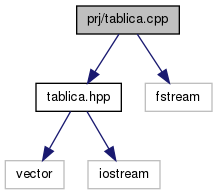
\includegraphics[width=235pt]{tablica_8cpp__incl}
\end{center}
\end{figure}


\subsection{Opis szczegółowy}
Definicja metody Dodaj\-Na\-Koniec. Definicja przeladowania operatora == .

Definicja przeladowania operatora = .

Definicja przeladowania operatora + .

Definicja metody Usun\-Ele.

Definicja metody Wyswietl\-Tab.

Definicja metody Pobierz\-Wskazany\-Ele.

Definicja metody Dodaj\-Na\-Miejsce.

Definicja metody Odwroc\-Tab.

Definicja metody zamien elementy.

Definicja metody Pobierz\-Rozmiar.

Definicja metody Pobierz\-Ostatni\-Ele.

Definicja metody Pobierz\-Pierwszy\-Ele.

Definicja metody Dodaj\-Na\-Poczatek.

Metoda, ktora dodaje na koniec element.

Metoda, ktora dodaje na poczatek element.

Metoda, ktora pobiera pierwszy element.

Metoda, ktora pobiera ostatni element.

Metoda, ktora pobiera pobiera rozmiar tablicy.

Metoda, ktora zamienia dwa wybrane elementy.

Metoda, ktora odwraca tablice.

Metoda, ktora dodaje element na konretne miejsce.

Metoda, ktora pobiera wskazany element.

Metoda, ktora wyswietla tabilce.

Metoda, ktora dusuwa elementy.

W celu lacznia dwoch tablic w jedna.

W celu przypisania dwoch tablic.

W celu lacznia porownania tablic. 

Definicja w pliku \hyperlink{tablica_8cpp_source}{tablica.\-cpp}.


\hypertarget{tablica_8hpp}{\section{Dokumentacja pliku C\-:/\-Users/\-Klijek/\-Desktop/\-L\-A\-B4/prj/tablica.hpp}
\label{tablica_8hpp}\index{C\-:/\-Users/\-Klijek/\-Desktop/\-L\-A\-B4/prj/tablica.\-hpp@{C\-:/\-Users/\-Klijek/\-Desktop/\-L\-A\-B4/prj/tablica.\-hpp}}
}


Definicja klasy \hyperlink{class_tablica}{Tablica}.  


{\ttfamily \#include $<$vector$>$}\\*
{\ttfamily \#include $<$iostream$>$}\\*
Wykres zależności załączania dla tablica.\-hpp\-:
Ten wykres pokazuje, które pliki bezpośrednio lub pośrednio załączają ten plik\-:
\subsection*{Komponenty}
\begin{DoxyCompactItemize}
\item 
class \hyperlink{class_tablica}{Tablica}
\end{DoxyCompactItemize}


\subsection{Opis szczegółowy}
Definicja klasy \hyperlink{class_tablica}{Tablica}. Klasa odpowiadaj�ca za operacje wykonujace sie na tablicy takie jak\-: zamienienie elementow, odwrocenie tablicy, dodanie elementu, dodanie elementow, operator + operator, operato == Oraz sortowania wykonywane dla stosu, a mianowicie quicksort, mergesort oraz heapsort. 

Definicja w pliku \hyperlink{tablica_8hpp_source}{tablica.\-hpp}.


\hypertarget{zegar_8cpp}{\section{Dokumentacja pliku prj/zegar.cpp}
\label{zegar_8cpp}\index{prj/zegar.\-cpp@{prj/zegar.\-cpp}}
}


Definicja metody Start.  


{\ttfamily \#include \char`\"{}zegar.\-hpp\char`\"{}}\\*
Wykres zależności załączania dla zegar.\-cpp\-:
\nopagebreak
\begin{figure}[H]
\begin{center}
\leavevmode
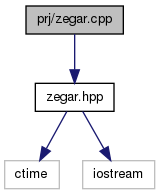
\includegraphics[width=192pt]{zegar_8cpp__incl}
\end{center}
\end{figure}


\subsection{Opis szczegółowy}
Definicja metody Start. Definicja metody Wynik.

Definicja metody Koniec.

Metoda, ktora powoduje start zegara.

Metoda, ktora powoduje stop zegara i oblicza czas.

Metoda, ktora wyswietla wynik. 

Definicja w pliku \hyperlink{zegar_8cpp_source}{zegar.\-cpp}.


\hypertarget{zegar_8hpp}{\section{Dokumentacja pliku prj/zegar.hpp}
\label{zegar_8hpp}\index{prj/zegar.\-hpp@{prj/zegar.\-hpp}}
}


Definicja klasy \hyperlink{class_tablica}{Tablica}.  


{\ttfamily \#include $<$ctime$>$}\\*
{\ttfamily \#include $<$iostream$>$}\\*
Wykres zależności załączania dla zegar.\-hpp\-:
\nopagebreak
\begin{figure}[H]
\begin{center}
\leavevmode
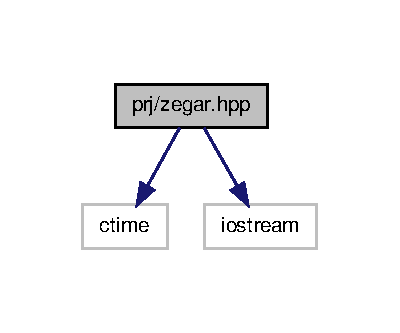
\includegraphics[width=192pt]{zegar_8hpp__incl}
\end{center}
\end{figure}
Ten wykres pokazuje, które pliki bezpośrednio lub pośrednio załączają ten plik\-:
\nopagebreak
\begin{figure}[H]
\begin{center}
\leavevmode
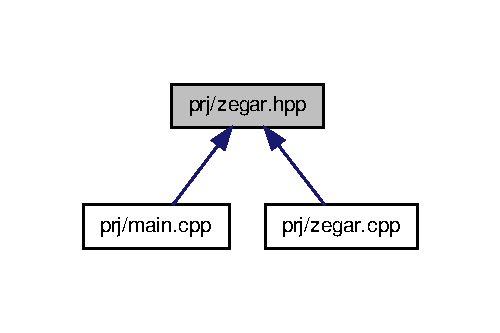
\includegraphics[width=240pt]{zegar_8hpp__dep__incl}
\end{center}
\end{figure}
\subsection*{Komponenty}
\begin{DoxyCompactItemize}
\item 
class \hyperlink{class_zegar}{Zegar}
\end{DoxyCompactItemize}


\subsection{Opis szczegółowy}
Definicja klasy \hyperlink{class_tablica}{Tablica}. Klasa odpowiadaj�ca za operacje wykonujace sie na tablicy takie jak\-: zamienienie elementow, odwrocenie tablicy, dodanie elementu, dodanie elementow, operator + operator, operato == 
\begin{DoxyParams}[1]{Parametry}
\mbox{\tt in}  & {\em clock\-\_\-t} & start, koniec -\/ zmienne przechowuja aktualny czas systemu \\
\hline
\mbox{\tt in}  & {\em czas} & -\/ przechowuje roznice czasow koniec i start \\
\hline
\end{DoxyParams}


Definicja w pliku \hyperlink{zegar_8hpp_source}{zegar.\-hpp}.


%--- End generated contents ---

% Index
\newpage
\phantomsection
\addcontentsline{toc}{chapter}{Indeks}
\printindex

\end{document}
